\documentclass[11pt,a4paper]{article}

\usepackage[margin=2.5cm]{geometry}
\usepackage{amsmath,amssymb}
\usepackage{booktabs}
\usepackage{graphicx}
\usepackage{tikz}
\usetikzlibrary{arrows.meta,positioning}
\usepackage[T1]{fontenc}
\usepackage[utf8]{inputenc}
\usepackage{microtype}
\usepackage{array}
\usepackage{tabularx}
\usepackage{hyperref}

\title{Dependency-order and preference-forest DP\\
differential compression of the gapped suffix array}
\author{}
\date{}

\begin{document}
\maketitle

\section{Setup and preliminaries}

\subsection{Gapped \(k\)-mers and DisLex}

Fix a binary shape \(S\) of \emph{span} \(s\) and \emph{weight} \(w\)
(number of care positions). On a DNA text \(T[0..n)\), every start
position \(p\) yields a gapped \(k\)-mer name
\(c = \mathrm{name}_S(T,p)\). For the running example we take
\[
T = (\mathtt{GCCTTTAAAG})^3,\qquad
|T|=n=30,\qquad
S=\mathtt{\#\,.\,\#},\qquad
s=3,\ w=2.
\]

The \textbf{DisLex} transform (Horton) lays these names out grouped by
residue class \(p\bmod s\), producing an integer string (the
\emph{lextext}) of length \(m=n+1=31\). Consecutive symbols inside a
residue class are exactly the successive windows
\(p,\ p+s,\ p+2s,\ldots\) --- i.e.\ the gapped suffix starting at
\(p\). The suffix array of the lextext is the \textbf{gapped suffix
array} (GSA); an LCP array is computed in symbol space (Kasai). Writing
\(\mathrm{sa}[r]\) for the lextext rank-\(r\) suffix and
\(\mathrm{orig}(r)\) for its original text start, the first symbol of
that suffix is the gapped \(k\)-mer at \(\mathrm{orig}(r)\).

\subsection{LCP intervals \(I_c\)}

Because the GSA is ordered by gapped suffixes, all ranks whose first
symbol equals a fixed name \(c\) form a contiguous interval
\[
I_c = [\ell_c,\, r_c)\subseteq\{0,\ldots,m-1\}.
\]
The multiset \(\{\mathrm{orig}(r):r\in I_c\}\) is precisely the sorted
list of text positions of \(c\). On the example, the intervals with
\(|I_c|>1\) are:

\begin{center}
\begin{tabular}{@{}llll@{}}
\toprule
\(c\) & SA range \(I_c\) & \(\lvert I_c\rvert\) &
  text positions \(\mathrm{orig}(\cdot)\) (rank order) \\
\midrule
AA & \([2,5)\)   & 3 & 26, 16, 6 \\
AG & \([5,10)\)  & 5 & 27, 18, 8, 17, 7 \\
CT & \([10,16)\) & 6 & 22, 21, 12, 2, 11, 1 \\
GC & \([17,22)\) & 5 & 19, 9, 20, 10, 0 \\
TA & \([22,28)\) & 6 & 25, 24, 15, 5, 14, 4 \\
TT & \([28,31)\) & 3 & 23, 13, 3 \\
\bottomrule
\end{tabular}
\end{center}

(Singletons \(\mathtt{\$\$}\), \(\mathtt{A\$}\), \(\mathtt{G\$}\) are
never differentially compressed.)

\subsection{Differential links}

Let \(x=\mathrm{sa}[r]\) be a lextext position. Shifting left by \(a\)
symbols in the lextext corresponds to walking \(a\) windows backward
along the same residue class. Whenever the alignment condition
\[
\mathrm{lex2orig}[x-a] = \mathrm{orig}(r) - a\cdot s
\]
holds, the suffix at \(x-a\) is a valid \textbf{left context} of depth
\(a\). Prepending \(a\) symbols preserves relative order among suffixes
and shifts original positions by \(+a\cdot s\).

Consequently, if a contiguous SA run \(J=[\sigma,\tau)\) has LCP depth
at least \(a+1\) and the symbol at depth \(a\) equals \(c\), then
mapping each kept source rank \(u\in J\) by
\[
\mathrm{orig}(u)\;\longmapsto\;\mathrm{orig}(u)+a\cdot s
\]
recovers, bijectively and in order, a subset of \(I_c\). We call
\((J,a)\) a \textbf{differential source} of coverage
\(\mathrm{cov}=|J'|\) for those covered ranks of \(I_c\).

\subsection{What is stored: \(C\), \(H_{\mathrm{offset}}\),
\(H_{\mathrm{rest}}\)}

Compression drops covered ranks from the stored position array. The
kept original positions, still in GSA rank order, form the compressed
array \(C\). For each name \(c\) the hash table stores at most two
entries:
\begin{itemize}
\item \(H_{\mathrm{offset}}=(\mathit{pos},\,a,\,\mathit{num})\):
  recover \(\mathit{num}\) positions as
  \(C[\mathit{pos}+t]+a\cdot s\) for \(t=0,\ldots,\mathit{num}-1\);
\item \(H_{\mathrm{rest}}=(\mathit{pos},\,\mathit{num})\):
  \(\mathit{num}\) positions stored directly in \(C\).
\end{itemize}
Ranks used as sources of an accepted link are \textbf{pinned} (their
pin-count increases) so that later decisions cannot remove them while
dependents still need them. The objective of source selection is to
minimise \(|C|\).

\section{The preference relation}

For each interval \(I_c\) with \(|I_c|>1\), the implementation
enumerates all viable sources for \(a=1,\ldots,a_{\max}\) (default
\(a_{\max}=8\)):
\begin{enumerate}
\item For every rank \(r\in I_c\), compute the predecessor lextext
  coordinate \(y=x-a\) if the alignment condition above holds; collect
  pairs \((\mathrm{rank}(y),\,r)\).
\item Sort by source rank and group into maximal contiguous runs where
  consecutive source ranks differ by~1 and \(\mathrm{LCP}\ge a+1\).
\item Retain a run only if it is \textbf{disjoint} from \(I_c\) and has
  coverage at least~3.
\end{enumerate}
Among all such candidates, the \textbf{preferred} candidate for
\(I_c\) maximises coverage, breaking ties by preferring larger \(a\)
(deeper LCP). Availability (pins~/ already-removed ranks) is
\emph{ignored} when building preferences: preference is a global,
static notion of ``who would like whom as differential source.''

Directionality is one-sided: sources always lie to the left in the
lextext (earlier windows on the same residue class). There is no
``forward'' differential link.

\section{The DepOrder algorithm}

DepOrder has three conceptual stages.

\subsection{Preference DAG}

For every interval with a preferred candidate of coverage \(\ge 3\),
draw a directed edge
\[
\text{source name}\;\longrightarrow\;\text{target name}
\]
meaning ``the target prefers a differential source inside the source's
interval.'' Self-loops are discarded. The resulting digraph may contain
cycles.

On the example the preferred candidates are:

\begin{center}
\begin{tabular}{@{}llllll@{}}
\toprule
target & prefers & \(a\) & cov & source SA range &
  covered ranks in target \\
\midrule
AA & \textbf{GC} & 2 & 3 & \([19,22)\) & \(\{2,3,4\}\) \\
AG & \textbf{CT} & 2 & 5 & \([11,16)\) & \(\{5,6,7,8,9\}\) \\
CT & \textbf{GC} & 4 & 2 & \([20,22)\) & \(\{10,12\}\) \\
GC & \textbf{CT} & 3 & 2 & \([14,16)\) & \(\{19,20\}\) \\
TA & \textbf{CT} & 1 & 6 & \([10,16)\) & \(\{22,\ldots,27\}\) \\
TT & \textbf{GC} & 1 & 3 & \([19,22)\) & \(\{28,29,30\}\) \\
\bottomrule
\end{tabular}
\end{center}

\begin{figure}[ht]
\centering
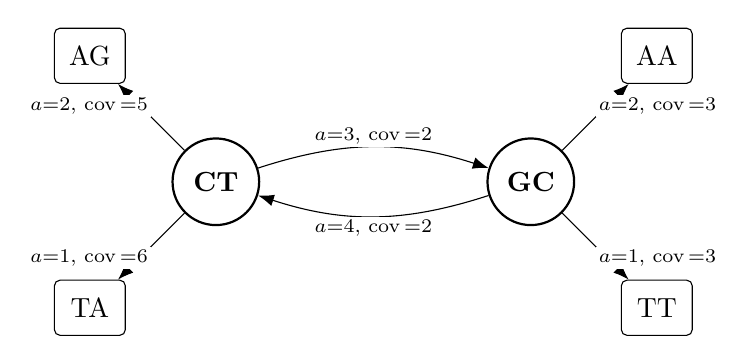
\begin{tikzpicture}[
  hub/.style={draw, thick, circle, minimum size=1.1cm,
              font=\bfseries},
  leaf/.style={draw, rounded corners=2pt, minimum width=0.9cm,
               minimum height=0.7cm},
  every edge/.style={draw, -{Latex[length=2mm]}},
  lbl/.style={font=\scriptsize, fill=white, inner sep=1pt}
]
  \node[hub]  (CT) at (0,0)  {CT};
  \node[hub]  (GC) at (4,0)  {GC};
  \node[leaf] (AG) at (-1.6,1.6) {AG};
  \node[leaf] (TA) at (-1.6,-1.6){TA};
  \node[leaf] (AA) at (5.6,1.6)  {AA};
  \node[leaf] (TT) at (5.6,-1.6) {TT};

  \draw (CT) edge[bend left=18]
    node[lbl, above] {\(a{=}3\), cov\({\,=}2\)} (GC);
  \draw (GC) edge[bend left=18]
    node[lbl, below] {\(a{=}4\), cov\({\,=}2\)} (CT);

  \draw (CT) edge node[lbl, above left] {\(a{=}2\), cov\({\,=}5\)} (AG);
  \draw (CT) edge node[lbl, below left] {\(a{=}1\), cov\({\,=}6\)} (TA);
  \draw (GC) edge node[lbl, above right]{\(a{=}2\), cov\({\,=}3\)} (AA);
  \draw (GC) edge node[lbl, below right]{\(a{=}1\), cov\({\,=}3\)} (TT);
\end{tikzpicture}
\caption{Preference DAG for
\(T=(\mathtt{GCCTTTAAAG})^3\), \(S=\mathtt{\#\,.\,\#}\).
An edge \(w\to c\) means that \(c\)'s preferred differential source
lies inside \(I_w\). Hubs CT and GC form a mutual-preference cycle;
leaves AA, TT, AG, TA are high-coverage dependents.}
\label{fig:pref-dag}
\end{figure}

\paragraph{Hubs.}
Both CT and GC are preferred sources for three names each. There is a
mutual preference cycle \(\mathrm{CT}\leftrightarrow\mathrm{GC}\). The
high-value dependents are the leaves AA, TT (via GC) and AG, TA (via
CT): together they offer coverage \(3+3+5+6=17\), while the hub--hub
edges themselves offer only coverage~2 each.

\subsection{Phase I --- reverse topological acceptance (sinks first)}

A Kahn topological order is computed on the preference DAG; remaining
nodes in any strongly connected component (here the CT--GC cycle and
its waiting dependents) are appended by decreasing interval size.
\textbf{Acceptance proceeds in reverse topological order}:
dependents~/ sinks before sources.

For each name in that order, the algorithm recomputes the best
candidate \emph{under current availability} (source run must be fully
kept; covered ranks must be free of pins and not already removed) and,
if coverage \(\ge 3\), accepts it: pin the source ranks, mark covered
ranks removed.

\paragraph{Why sinks first helps hubs.}
Accepting a leaf that points into a hub pins the hub's ranks before
the hub itself is considered. A hub that would like to compress
\emph{itself} away (using the other hub) then finds its own ranks
already pinned and is forced to \textbf{skip}, remaining available as
a source for all dependents. Size-first greedy does the opposite: it
lets a large hub claim a weak slice of another hub early, spoiling
high-coverage leaf links.

\subsection{Phase II --- unpin~/ retarget with transitive add}

After Phase~I, a fixed-point pass repeatedly tries, for intervals in
decreasing size order, candidates of \emph{strictly larger} coverage
than the current acceptance --- temporarily ignoring pin constraints
on covered ranks. Accepting such a candidate may require
\textbf{retargeting} dependents that currently pin those ranks: if a
dependent \(D\)'s source run is a contiguous sub-run of the new
candidate's covered ranks, \(D\) is rewritten to point at the
corresponding sub-run of the new source with
\[
a'_D = a_D + a_{\mathrm{new}}.
\]
The attempt is transactional (snapshot~/ rollback) and kept only if
the global number of kept ranks decreases, or coverage for that name
improves. Phase~II is where former sources can themselves be
compressed once their dependents have been lifted onto a deeper
source.

\section{Worked example:
\(\mathtt{GCCTTTAAAG}{\times}3\) with \(\mathtt{\#\,.\,\#}\)}

Parameters: \(n=30\), \(s=3\), \(m=31\), \(a_{\max}=8\). Distinct
names:~9.

\subsection{Phase I on the example}

Because of the CT--GC cycle, Kahn's order first drains the
indegree-\(0\) singletons, then appends the cyclic component by size.
Reverse-topo acceptance among compressible names is
\[
\mathrm{TT},\;\mathrm{AA},\;\mathrm{GC},\;\mathrm{AG},\;
\mathrm{TA},\;\mathrm{CT}.
\]

\begin{center}
\small
\begin{tabular}{@{}cllp{7.6cm}@{}}
\toprule
step & interval & decision & detail \\
\midrule
I.1 & TT & \textbf{ACCEPT} &
  \(\leftarrow\) GC\([19,22)\), \(a=1\), cov\({=}3\).
  Pins GC ranks 19--21. \\
I.2 & AA & \textbf{ACCEPT} &
  \(\leftarrow\) GC\([19,22)\), \(a=2\), cov\({=}3\).
  Same hub pins reinforced. \\
I.3 & GC & \textbf{SKIP} &
  Preferred source CT\([14,16)\) would cover GC ranks \(\{19,20\}\),
  but those ranks are already pinned by TT/AA. Availability blocks
  self-compression of the hub. \\
I.4 & AG & \textbf{ACCEPT} &
  \(\leftarrow\) CT\([11,16)\), \(a=2\), cov\({=}5\).
  Pins CT ranks 11--15. \\
I.5 & TA & \textbf{ACCEPT} &
  \(\leftarrow\) CT\([10,16)\), \(a=1\), cov\({=}6\).
  Pins full CT hub. \\
I.6 & CT & \textbf{SKIP} &
  Preferred GC\([20,22)\) is pinned; covered CT ranks are themselves
  pinned as sources. Hub preserved. \\
\bottomrule
\end{tabular}
\end{center}

After Phase~I: \textbf{kept \({=}14\)}, four accepted offsets
(AA, AG, TA, TT). Phase~II finds no improving retarget on this
instance, so the final size remains \(|C|=14\).

Explicitly, \(C\) stores the three singletons plus the entire hubs CT
and GC:
\[
C = [30,\,28,\,22,\,21,\,12,\,2,\,11,\,1,\,29,\,19,\,9,\,20,\,10,\,0].
\]

Hash table (offset~/ rest):

\begin{center}
\begin{tabular}{@{}lll@{}}
\toprule
\(c\) & \(H_{\mathrm{offset}}\) & \(H_{\mathrm{rest}}\) \\
\midrule
\$\$ & --- & \((0,1)\) \\
A\$ & --- & \((1,1)\) \\
AA & \((11,\,2,\,3)\) & --- \\
AG & \((3,\,2,\,5)\)  & --- \\
CT & --- & \((2,\,6)\) \\
G\$ & --- & \((8,\,1)\) \\
GC & --- & \((9,\,5)\) \\
TA & \((2,\,1,\,6)\)  & --- \\
TT & \((11,\,1,\,3)\) & --- \\
\bottomrule
\end{tabular}
\end{center}

All 17 non-hub, non-singleton positions are recovered from the two
hubs: \(3+5+6+3=17\), and \(31-17=14\).

\subsection{Contrast: size-order greedy (\(|C|=22\))}

Greedy processes intervals by decreasing \(|I_c|\), with availability,
and pins sources permanently:
\begin{enumerate}
\item \textbf{CT} (size~6) accepts GC\([20,22)\), \(a=4\), cov only
  \textbf{2} --- a weak use of two GC hub ranks to drop two of six CT
  positions.
\item \textbf{TA} (size~6) is then limited to the same spoiled GC
  slice: cov only \textbf{2}.
\item \textbf{AG} (size~5) \textbf{skips} --- its preferred CT source
  is no longer fully available.
\item \textbf{GC} falls back to TT\([29,31)\), \(a=2\), cov
  \textbf{2}.
\item \textbf{AA} still accepts GC\([19,22)\), cov~3.
\item \textbf{TT} \textbf{skips}.
\end{enumerate}
Net removal: \(2+2+2+3=9\) ranks, hence \(|C|=22\). The structural
mistake is clear: by letting the hub CT claim a low-coverage fragment
of GC first, greedy destroys the high-coverage leaf edges (AG cov~5,
TA cov~6, TT cov~3) that DepOrder's sinks-first order realises in
full.

\begin{center}
\begin{tabular}{@{}lrr@{}}
\toprule
algorithm & \(|C|\) & fraction of \(m=31\) \\
\midrule
Greedy   & \textbf{22} & 71.0\% \\
DepOrder & \textbf{14} & 45.2\% \\
\bottomrule
\end{tabular}
\end{center}

(On this instance Greedy-DFS reaches~15 --- better than greedy, still
one above DepOrder.)

\section{Complexity and when DepOrder helps}

Phase~I is a single pass over a topological (or size-refined) order,
each step re-enumerating candidates for one interval --- inexpensive
relative to GSA construction. Phase~II may repeat enumeration,
snapshotting, and retarget attempts over \(O(N)\) rounds
(\(N=\#\) intervals) and is the asymptotic bottleneck on large
instances; on the present toy example it is a no-op.

DepOrder helps precisely when the preference graph has \textbf{high
fan-out hubs} whose own preferred self-compression edges are
low-coverage, while many dependents offer large coverage into those
hubs. Sinks-first pinning protects the hubs; Phase~II's transitive add
is reserved for the harder case where a hub should later be compressed
\emph{through} a deeper source after dependents have been retargeted.
The \(\mathtt{GCCTTTAAAG}{\times}3\)~/ \(\mathtt{\#\,.\,\#}\) instance
is the minimal didactic witness of the hub-protection phenomenon: CT
and GC must stay in \(C\), and every other multi-occurrence name
collapses onto them, yielding \(|C|=14\) against greedy's \(22\).

\section{The Tree-DP algorithm
(preference-forest DP)}

Tree-DP attacks the same objective --- minimise \(|C|\) --- by an exact
dynamic program on a \emph{preference forest} extracted from the same
static preferences, followed by the shared Phase~II pass.

\subsection{From preference DAG to preference forest}

Recall that each interval \(I_c\) with \(|I_c|>1\) has a preferred
differential candidate (maximising coverage, then \(a\)). Tree-DP
retains a candidate for name \(c\) only if
\[
|I_c|>2
\]
(singletons and size-\(2\) intervals are left to a later leftover
pass). A directed preference \(w\to c\) (``\(c\) prefers a source
inside \(I_w\)'') becomes a \textbf{forest edge} only when its
coverage satisfies
\[
\mathrm{cov}\ge 3.
\]
Self-loops are dropped, and an edge is skipped if it would close a
cycle in the forest under construction. The resulting graph is
therefore a forest of rooted trees: each non-root \(c\) has a unique
parent \(\mathrm{parent}(c)=w\), the preferred source of \(c\).

Weak mutual preferences of coverage~$2$ (such as
\(\mathrm{CT}\leftrightarrow\mathrm{GC}\) on the running example) are
filtered out by the \(\mathrm{cov}\ge 3\) threshold, so cycles in the
full preference DAG typically dissolve into independent high-coverage
stars.

\subsection{KEEP versus COMPRESS}

Write \(\mathrm{isize}(v)=|I_v|\). For a node \(v\) whose preferred
source is currently available (\(\mathit{src\_ok}=\mathsf{true}\)),
Tree-DP chooses between two local decisions:

\begin{itemize}
\item \textbf{KEEP} \(v\): store all \(\mathrm{isize}(v)\) ranks of
  \(I_v\). Every child \(w\) may then treat \(v\) as an available
  source:
  \[
  \mathrm{cost}_{\mathrm{keep}}(v)
  =
  \mathrm{isize}(v)
  +
  \sum_{w\,\mathrm{child\,of}\,v}
    \mathrm{DP}(w,\,\mathit{src\_ok}=\mathsf{true}).
  \]
\item \textbf{COMPRESS} \(v\): accept the preferred candidate of
  coverage \(\mathrm{cov}(v)\), paying only the uncovered ranks
  \(\mathrm{isize}(v)-\mathrm{cov}(v)\). Children lose \(v\) as a
  source:
  \[
  \mathrm{cost}_{\mathrm{comp}}(v)
  =
  \mathrm{isize}(v)-\mathrm{cov}(v)
  +
  \sum_{w\,\mathrm{child\,of}\,v}
    \mathrm{DP}(w,\,\mathit{src\_ok}=\mathsf{false}).
  \]
\end{itemize}
The recurrence returns the cheaper option (KEEP on a tie). If
\(\mathit{src\_ok}=\mathsf{false}\), COMPRESS is forbidden and the
node is forced to KEEP. Roots are handled identically, except that
COMPRESS is allowed only when the preferred source lies
\emph{outside} the root's preference subtree (so the source is not
itself a forest descendant of the root).

The DP is exact for the \(|C|\) contribution of all forest nodes under
this KEEP~/ COMPRESS model. Intervals that never entered the forest
(or remain uncompressed after the DP choice) are finished by a
size-ordered availability greedy; then the shared Phase~II
unpin~/ retarget fixed point of DepOrder is run unchanged.

\subsection{Worked example on the preference forest}

On \(T=(\mathtt{GCCTTTAAAG})^3\), \(S=\mathtt{\#\,.\,\#}\), the
\(\mathrm{cov}\ge 3\) filter retains exactly four edges and yields two
stars:

\begin{center}
\begin{tabular}{@{}llll@{}}
\toprule
parent (source) & child (target) & \(a\) & cov \\
\midrule
GC & AA & 2 & 3 \\
GC & TT & 1 & 3 \\
CT & AG & 2 & 5 \\
CT & TA & 1 & 6 \\
\bottomrule
\end{tabular}
\end{center}

\begin{figure}[ht]
\centering
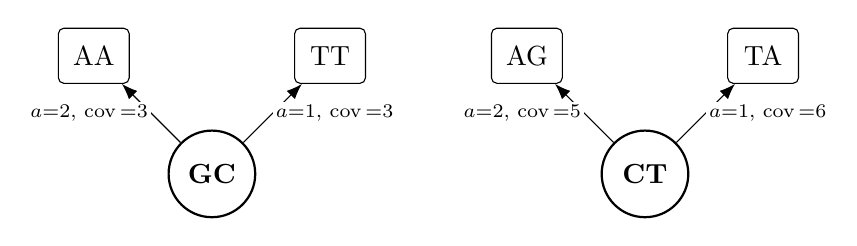
\begin{tikzpicture}[
  hub/.style={draw, thick, circle, minimum size=1.1cm,
              font=\bfseries},
  leaf/.style={draw, rounded corners=2pt, minimum width=0.9cm,
               minimum height=0.7cm},
  every edge/.style={draw, -{Latex[length=2mm]}},
  lbl/.style={font=\scriptsize, fill=white, inner sep=1pt}
]
  \node[hub]  (GC) at (0,0)  {GC};
  \node[leaf] (AA) at (-1.5,1.5) {AA};
  \node[leaf] (TT) at (1.5,1.5)  {TT};

  \node[hub]  (CT) at (5.5,0)  {CT};
  \node[leaf] (AG) at (4.0,1.5) {AG};
  \node[leaf] (TA) at (7.0,1.5) {TA};

  \draw (GC) edge node[lbl, left]  {\(a{=}2\), cov\({\,=}3\)} (AA);
  \draw (GC) edge node[lbl, right] {\(a{=}1\), cov\({\,=}3\)} (TT);
  \draw (CT) edge node[lbl, left]  {\(a{=}2\), cov\({\,=}5\)} (AG);
  \draw (CT) edge node[lbl, right] {\(a{=}1\), cov\({\,=}6\)} (TA);
\end{tikzpicture}
\caption{Preference forest for the running example: two stars
\(\mathrm{GC}\to\{\mathrm{AA},\mathrm{TT}\}\) and
\(\mathrm{CT}\to\{\mathrm{AG},\mathrm{TA}\}\). The weak hub--hub
edges of coverage~$2$ do not enter the forest.}
\label{fig:pref-forest}
\end{figure}

\paragraph{Leaves under an available hub.}
With \(\mathit{src\_ok}=\mathsf{true}\), each leaf prefers COMPRESS:
e.g.\ \(\mathrm{cost}_{\mathrm{comp}}(\mathrm{AA})=3-3=0\)
(versus KEEP~$3$), and likewise TT, AG, TA all compress to cost~$0$.

\paragraph{Root GC.}
\[
\begin{aligned}
\mathrm{cost}_{\mathrm{keep}}(\mathrm{GC})
  &= 5 + 0 + 0 = 5,\\
\mathrm{cost}_{\mathrm{comp}}(\mathrm{GC})
  &= (5-2) + \underbrace{3}_{\mathrm{AA\,KEEP}}
           + \underbrace{3}_{\mathrm{TT\,KEEP}} = 9
\end{aligned}
\]
(compressing GC via CT would deny the children their hub, forcing
them to KEEP). Since \(5<9\), the DP \textbf{KEEPs} GC.

\paragraph{Root CT.}
\[
\begin{aligned}
\mathrm{cost}_{\mathrm{keep}}(\mathrm{CT})
  &= 6 + 0 + 0 = 6,\\
\mathrm{cost}_{\mathrm{comp}}(\mathrm{CT})
  &= (6-2) + 5 + 6 = 15.
\end{aligned}
\]
Again KEEP wins. Materialisation accepts the four leaf compressions
(deepest first), leftover greedy finds nothing further, and Phase~II
is a no-op --- exactly as under DepOrder --- yielding
\[
|C|=14.
\]

\subsection{Contrast with DepOrder}

Both algorithms protect the same hubs on this instance and reach the
same \(|C|=14\). They differ in mechanism:

\begin{center}
\small
\begin{tabular}{@{}p{2.8cm}p{5.6cm}p{5.6cm}@{}}
\toprule
 & DepOrder & Tree-DP \\
\midrule
Graph model &
  preference DAG (cycles allowed) &
  preference forest:
  nodes with \(|I_c|>2\);
  edges only if \(\mathrm{cov}\ge 3\)
  (cycle-breaking) \\
Phase~I &
  reverse-topo acceptance with live
  availability~/ pins (sinks first) &
  exact KEEP~/ COMPRESS DP per tree;
  materialise deepest-first \\
Hub--hub cov~$2$ &
  present in the DAG; sinks-first
  pinning forces hubs to SKIP &
  omitted from the forest; DP compares
  \(\mathrm{cost}_{\mathrm{keep}}\)
  (\(5\)~/ \(6\)) to the costly COMPRESS
  alternative \\
Phase~II &
  unpin~/ retarget~/ transitive add &
  same shared Phase~II \\
\bottomrule
\end{tabular}
\end{center}

DepOrder reasons operationally (who pins whom, in which order).
Tree-DP reasons globally on a simplified forest: the numeric comparison
\(\mathrm{cost}_{\mathrm{keep}}<\mathrm{cost}_{\mathrm{comp}}\) is
precisely the statement that keeping a hub is cheaper than
compressing it at the expense of its high-coverage dependents --- the
same structural insight DepOrder realises by sinks-first pinning.

\section{Summary}

On the didactic instance
\(\mathtt{GCCTTTAAAG}{\times}3\)~/ \(\mathtt{\#\,.\,\#}\), both
DepOrder and Tree-DP store the hubs CT and GC in full, differentially
recover AA, TT, AG, and TA from them, and finish at \(|C|=14\)
(against size-order greedy's~$22$). Phase~II is common to both and
idle here; it matters when a kept hub should later be lifted onto a
deeper source after dependents have been retargeted. Tree-DP's
filters \(|I_c|>2\) and \(\mathrm{cov}\ge 3\) turn the cyclic
preference DAG into a clean two-star forest on which KEEP versus
COMPRESS is decided by dynamic programming.

\end{document}
